\chapter{Introduction}
\label{chp:introduction}

It is the challenge that almost every software project faces at one point: bottlenecks.
Bottlenecks can lead to reduced speed, increased memory consumption, reduced responsiveness of a program or hampers the scalability of the project.
Each of these manifest in a reduction of user experience.
An example can be found in Google Chrome that is known for its speed.
It is also known for it extreme RAM consumption which leads to issues on older devices.

Over the course of years, profilers have been introduced to allow developers to profile their running code.
By inspecting the data generated by these profilers, developers can pinpoint functions that are consuming e.g. a lot of wall- or CPU time which may indicate a bottleneck is present.
Additionally, once a bottleneck has been resolved it can be verified by using a profiler that it indeed does consume less resources, i.e. time or memory.

However, in large and complex systems there are likely to be many bottlenecks present.
J. M. Juran's Pareto principle admonishes that one should "Concentrate on the vital few, not the trivial many" . This principle is also known as the 80/20 rule. \todo{cite paper and explain more.}

In this thesis we use the BitTorrent client Tribler as a use case to find and resolve bottlenecks.
Tribler has been in development for over ten years and has grown into a highly complex and distributed system.
The remainder of this chapter is used to introduce Tribler and its components as well as providing the outline of this thesis.

\section{Tribler}
Tribler is a peer-to-peer BitTorrent client that attempts to fully decentralize downloading, uploading and streaming of content while providing anonymity to its users.

Tribler focuses on the following goals:
\begin{itemize}
    \item Allow for secure and private communication and sharing of data.
    \item Enforce user contribution in the network by making use of the Multi-Chain.
    \item Reward seeding of poorly-seeded content by using credit mining.
    \item Make it impossible to shut Tribler down, unless the Internet itself as a whole gets taken down.
\end{itemize}

A fully decentralized ecosystem i.e. no central components present, is Tribler's approach to achieve these goals.
Tribler has been designed and build with this focus~\cite{Pouwelse-tribler,Bakker-tribler}.
A distributed network requires both the presence and collaboration of participants, called peers, to be able to achieve this.

% \begin{figure}
%	\centerline{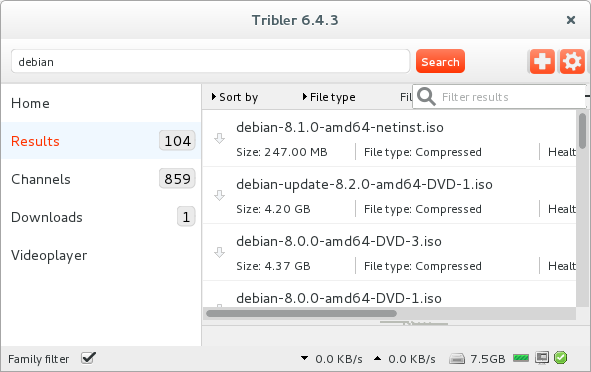
\includegraphics[scale=0.6]{introduction/figs/tribler-screenshot.png}}
%	\caption{Screenshot of Tribler v6.4.3.}
%	\label{fig:tribler-screenshot}
%\end{figure}

For years Tribler has received many contributions from students, staff and the open-source community.
However, adhering to one programming style and structure was never enforced.
\todo{I think the text below is more or less problem description. Should be removed and write what Tribler is about and more details.}
This led to the degradation of structure and code quality of the Tribler code base.
Moreover, there has been done little profiling to detect bottlenecks in the code.
Finding and resolving bottlenecks in a complex code base such as Tribler's are often non-trivial yet an excellent way to increase responsiveness and performance.
For example, performing a blocking network request to a non or poorly responsive server can make the whole program grind to a halt, rendering the GUI non-responsive and leaving the user guessing what happened.
By making such a request non-blocking, the GUI remains responsive while the request is handled in the background.
In the meantime, changing such a request to become non-blocking goes well with refactoring the current structure and quality of the code to become a coherent, well-tested whole.\\

Another motivating example can be found in a recent addition to Tribler's code base.
Within Tribler anonymous connections have been recently implemented using onion routing~\cite{Plak-anonymous,ruigrok-anonymous,tanaskoski-anonymous}.
These anonymous connections are called anon-tunnels in Tribler.
This feature allows users to anonymously download files from other users in the network, safeguarding their privacy.
Every data packet has to be encrypted with multiple encryption layers and forwarded by a number of intermediate hops between the leecher and seeder~\cite{Plak-anonymous,tanaskoski-anonymous}, each decrypting one layer of encryption.
The total cost of bandwidth per file is increased, because it has to be forwarded by multiple nodes.
Because a node in the network may become part of an anon-tunnel, the workload increases per node.
The anon-tunnels have been profiled by [stokkink et al.] \todo{cite to stok et al.} and the results showed that the tunnels are now bound by CPU.
As handling packets involves encryption or decryption and message serialization, which are CPU intensive tasks, one wants to optimize this process.
The result should be higher achievable download rates and a more responsive program.

\section{Dispersy}
The Distributed Permission System (Dispersy) is an elastic database system written in the Python programming language and uses SQLite as its underlying database engine.
It is designed to still function when faced with challenging network conditions such as low internet speed, connection drops, package loss and even when hurdles such as firewalls are in place.
Additionally, Dispersy is built to scale very well; over 100.000 bundles can be handled by Dispersy.
It workings have been proven throughout the years as it's heavily used within the Tribler client and is maintained by the Tribler organisation.

In Dispersy one can define communities in which peers can send messages to each other.
Every community and peer is uniquely identified and secured by making use of elliptic curve cryptography.
By performing peer exchanges (PEX) and by making use of Distributed Hash Tables (DHT's), peers receive continuously information about the network.

One of Dispersy's unique points is that it does not rely on a central component with the exception of bootstrap servers.
Furthermore, Dispersy's main features are:
\begin{itemize}
	\item Stateless synchronization using Bloomfilters.
	\item Decentralized NAT traversal.
	\item Performance that can scale to over 100,000 bundles.
\end{itemize}


\todo{more explanation needed.}
\section{Outline}
In this chapter we provided an introduction of this thesis and presented the research questions this thesis aims to answer. 
This section describes the other chapters in this thesis and their relevance to the research questions provided in section \ref{chp1:sct:objectives-research-questions}.
Chapter \ref{chp:preliminaries} provides preliminaries and terminology used through this thesis.
Chapter \ref{chp:problem-description} presents an overview of some of the problems Tribler is currently facing which this thesis addresses.
Chapter 
\todo{Add more here as cahpters are added.}
